\documentclass[fontsize=11pt]{article}
\usepackage{amsmath}
\usepackage[utf8]{inputenc}
\usepackage[margin=0.75in]{geometry}
\usepackage[
    backend=biber,
    style=apa,
]{biblatex}
\usepackage{graphicx}
\usepackage{hyperref}

\hypersetup{
    colorlinks=true,
    urlcolor=blue,
    citecolor=black,
}
\urlstyle{same}

\addbibresource{references.bib}

\title{CSC110 Project Report: COVID-19 Economics}
\author{Jacob Kolyakov, Theodore Preduta}
\date{Tuesday, December 14, 2021}

\begin{document}
\maketitle

\section*{Introduction}

In March 2020 the S\&P 500, an American index that is synonymous with its stability of growth experienced its sharpest decline in value since the housing market crash in 2008 (\cite{yahoo}).
At the same time the United States experienced its first major wave of COVID-19 cases and was forced into lockdown. 
When we saw the initial sharp decline of the S\&P 500 correlated with the time when COVID-19 cases first exploded in the United States, we hypothesized that there might be a connection between COVID-19 cases and the decline in value.
Since March 2020, there have been several more small yet sharp declines in both the S\&P 500 and TX60 (Canada's largest index) prices as COVID-19 case numbers fluctuated in the United States, which raises the question:
\textbf{To what degree do changes in COVID-19 case numbers in Canada, the United States and China correlate to changes in the Canadian and American economy as measured by change in stock indices?}
This question arose because compared to individual stocks, which are a microcosm of the economy, indices track the performances of a collection of stocks that are considered to represent a section of the stock market/economy (\cite{indexesgov}). 
The fact that the S\&P500 and TX60 had a sharp decline indicated to us that not only did COVID-19 affect certain stocks but the economies of the United States and Canada as a whole. 
We choose to explore different countries to see whether there is a significant degree of correlation and how that value differs when comparing Covid-19 cases for different countries to each economy and what that might say about the effectiveness of countries' strategies in handling the COVID-19 pandemic.
The United States is also an interesting case to look at as they gave out relief money during the pandemic, a portion of which may have been invested into the S\&P 500 and influencing its trends.
This in turn, possibly, might have lessened the degree of which COVID-19 case numbers impacted the economy.

\section*{Dataset Description}

This project relies on three data sources, two for financial data, and one for COVID-19 data.
The COVID-19 data comes from Our World in Data which contains global COVID-19 data as a CSV, licensed under CC-BY (\cite{owidcoronavirus}).
The data gets split into separate files by country each named \texttt{covid-<country code>.csv} for the three country codes (\texttt{can}, \texttt{chn}, \texttt{usa}).
In each file we only keep two columns, the date and the new cases reported in that country on that day.
So the data in \texttt{covid-can.csv} looks like:

\begin{center}
\begin{tabular}{|l|l|}
    \hline
    Date & New Cases \\
    \hline
    2020-06-25 & 324 \\
    2021-03-19 & 4274 \\
    \hline
\end{tabular}
\end{center}

The financial data for the S\&P500 is found through Yahoo Finance data, publicly available, as a CSV, through their API (\cite{yahoo}).
Similarly the financial data for the TX60 if found through investing.com, publicly available, as a CSV, through their API (\cite{investing.com}).
They are each stored in a file named \texttt{stock-<ticker>.csv} for each stock (\texttt{snp500} and \texttt{tx60}).
The columns provided are the Date, and the Open/High/Low/Close prices.
So the data in \texttt{stock-snp500.csv} looks like:

\begin{center}
\begin{tabular}{|l|l|l|l|l|}
    \hline
    Date & Open & High & Low & Close \\
    \hline
    2021-01-04 & 3764.610107421875 & 3769.989990234375 & 3662.7099609375 & 3700.64990234375 \\
    2021-04-19 & 4179.7998046875 & 4180.81005859375 & 4150.47021484375 & 4163.259765625 \\
    \hline
\end{tabular}
\end{center}


\section*{Computational Overview}

We analyzed the direct impact of COVID-19 case numbers on the chosen stock market in using two separate methods each having their own assumptions (these assumptions will be further elaborated upon in the discussion section).
We have dubbed these two strategies the `global' and `local' trends.
Both the global and the local trend analyses only look at a single COVID-19 data set and a single stock data set at a time, for example a single global analysis could compare the COVID-19 data of Canada against the close stock data of the TX50.

Before doing any analysis of the data, we first transform the data in each CSV file into a list of \texttt{float} or \texttt{int} depending on the type of data.
We do this by starting with array of all zeroes, and placing the relevant values in that list at the index of the number of days between that data point and the start date of the analysis.
This ensures that for the rest of the program we can make the assumption that the length of all data sets are equal, and the date at one index will be the same in each data set.

In the global trend analysis, we `shift' the timing of the COVID-19 data forward by between 0 and 90 days by removing the first days elements, and we trim the relevant stock data so that both lists of data are the same length.
Then we calculate the correlation coefficient for this new set of data.

In the local trend analysis, we only want to look at `spikes' of COVID-19 and stock data.
First we must find the threshold of what we consider to be a spike, which we consider to be the average of the magnitude of the data (either COVID-19 or stock) with the zero values dropped from the list (justification in the discussion section).
We then align spikes in the COVID-19 data with spikes in the stock data provided that the COVID-19 spike is within a user-configurable max difference value (otherwise the resulting spike is matched up with 0).
With this new data set of matched spikes between a set of COVID-19 and stock data, we can calculate its correlation coefficient.

The backbone of the above two systems is the \texttt{pandas.Series.corr} function which can compute the correlation coefficient which is a mathematical measure of how close two sequences of data correlate (\cite{pandaseriescorr}).
The relevant data is first transformed from two \texttt{list}s to a single \texttt{list} of \texttt{tuple}s each containing two values (the two values that are in the original list at that index).
This data form of the data can be used to construct a \texttt{pandas.DataFrame} which is a subclass of \texttt{pandas.Series} on which the correlation coefficient can be calculated (\cite{pandaseries}).
The correlation coefficient produced will be a value between -1 and 1, where the closer the value is to 1, the higher the probability of a positive direct correlation and likewise with -1 and a negative direct correlation (\cite{pandaseriescorr}).

Visualizing the data is a combination of the Plotly library and one of its extensions, Dash.
Plotly itself is only responsible for producing the graphs, while Dash allows dynamic updates.
We created the application as a single web page with both graphs on it.
We use the \texttt{dash.Dash.callback} function to setup our update functions to render a new graph when the input is changed in the relevant components (\cite{dash}).

\section*{Usage Instructions}

\begin{enumerate}
    \item Install the requirements in \texttt{requirements.txt} either using the PyCharm GUI or by running \texttt{pip install -r requirements.txt} in the command line.
    
    \item The raw COVID-19 data can be downloaded \href{https://github.com/owid/covid-19-data/blob/master/public/data/owid-covid-data.csv}{here}, the raw data for the S\&P500 can be downloaded \href{https://finance.yahoo.com/quote/\%5EGSPC/history?p=\%5EGSPC}{here}, and the raw data for the TX60 can be downloaded \href{https://ca.investing.com/indices/s-p-tsx-60-historical-data}{here}, however we processed the data into a more convenient form for the program.
    
    Download the final processed data from UTSend \href{http://REDACTED}{here}, or with the following information:
    
    \begin{center}
    \begin{tabular}{|c|c|}
        \hline
        Claim ID & REDACTED \\
        \hline
        Claim Passcode & REDACTED \\
        \hline
    \end{tabular}
    \end{center}
    
    And place the five files named \texttt{stock-*.csv}/\texttt{covid-*.csv} in a folder named \texttt{data} (where the \texttt{data} folder is in the same directory as \texttt{main.py}).
    
    \item Run \texttt{main.py}!
    Then open your browser to \texttt{http://localhost:8050}.
    The results from running main.py should look something similar to the following:
    
    \begin{center}
        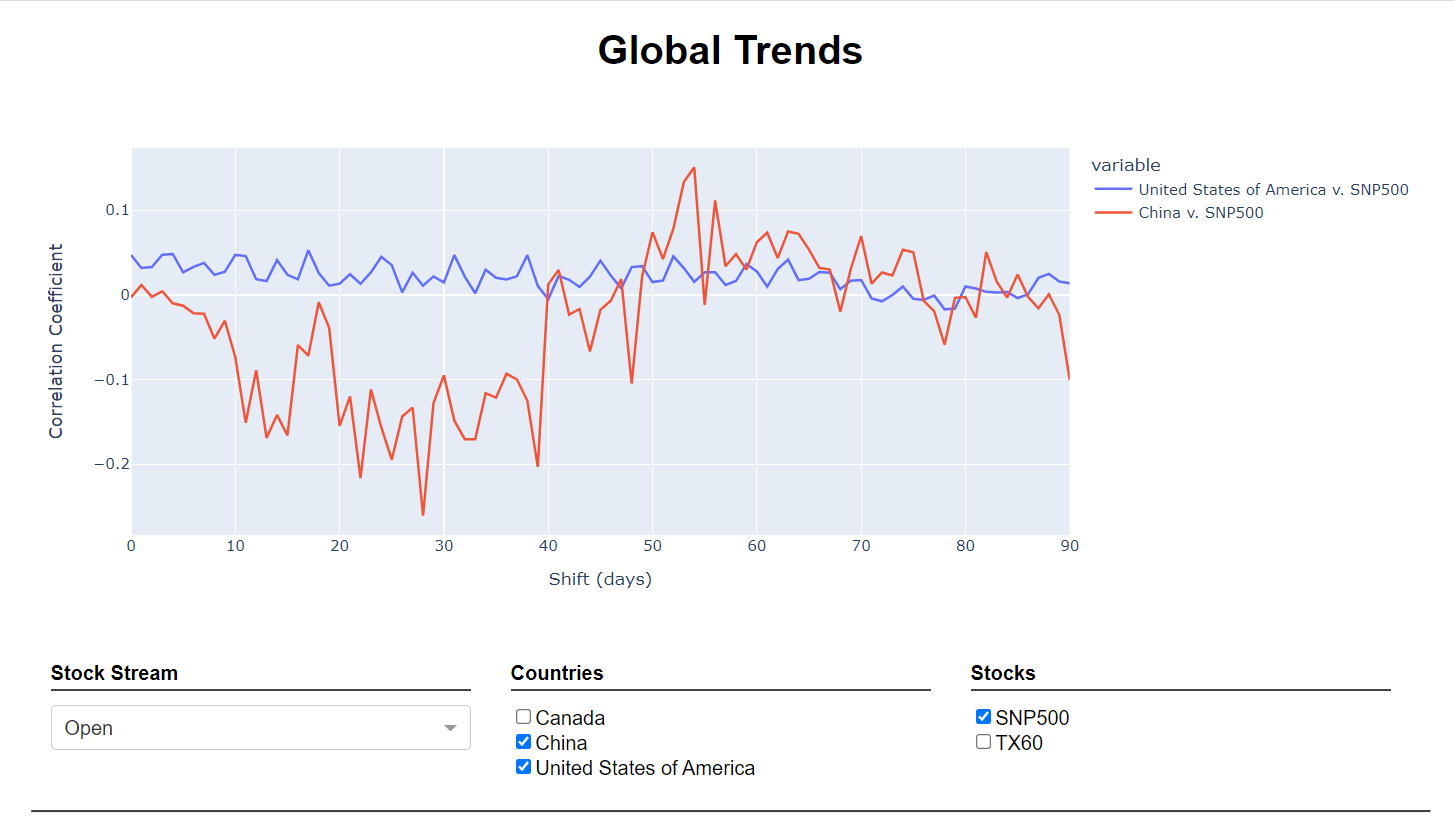
\includegraphics[scale=0.25]{global.png}\\
        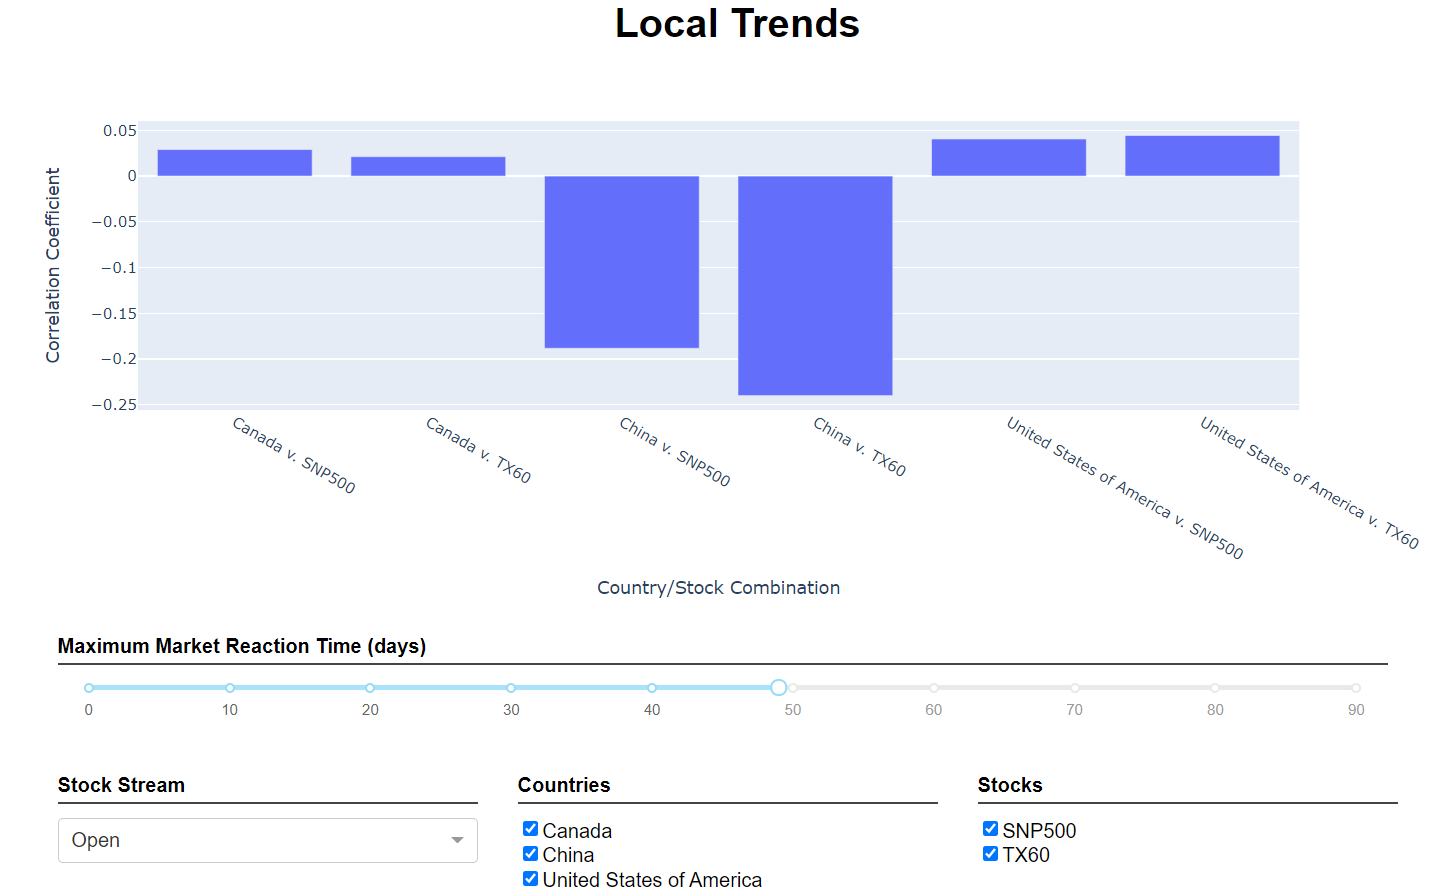
\includegraphics[scale=0.25]{local.png}
    \end{center}
    
    \item Now you can alter what kind of data you are seeing. For both graphs, the drop-down menu will change what stock values are being considered in the graph.
    `open' represents the value of the stock at beginning of each day, `close' represents the value of the stock at the end of each day and `high' and `low' represent the highest and lowest values of the stock each day.
    The checkboxes under countries will include or exclude the COVID-19 data from that country in the represented graph. The same is applicable happen with both stock indexes.
    
    Note the second graph has a slider below it.
    This slider allows you to change the maximum amount of time after a COVID-19 spike that a stock spike is considered correlated and will be included in the calculations. 
\end{enumerate}

\section*{Changes}

Firstly, we added a Canadian stock indicator to our roster of stocks to compare two.
By doing so, we can make conclusions about both Canada and the USA, instead of just the USA.

Secondly, we decided not to find the number of days between a COVID-19 spike and a stock spike.
By finding the average number of days between a COVID-19 spike and a stock spike, we have to assume that there already exists a causation relationship between the COVID-19 data and the stock data, however the question we want to answer is whether such a relationship exists.
So by finding this value, we do not get any closer to answering the research question.

Finally we decided to automatically find the threshold for a spike in the COVID-19 data and a separate one for the stock data instead of allowing the user to chose that value.
Let's assume that we find a set of values that produces a statistically significant result, it would be nearly impossible to justify why that specific pair of numbers allows us to make conclusions about the entire data set.
Instead, we start with a justifiable value and see if our prediction about it is correct.
We allow the user to vary the maximum reaction time, which can justified if a strong result emerged (one did not).

\section*{Discussion}

We chose for our results to be in the form of correlation coefficients.
This is because we believed that a statistically significant correlation coefficient would be a good indicator of a possible high degree of correlation between COVID-19 case numbers and the Canadian and American economies.

First, we defined what we considered a spike in stock value and a spike in COVID-19 case numbers to look like as these are both values that filter the data being considered in calculating the correlation coefficient. 
We chose these by finding the `inflated' average (the average excluding all 0 values). 
We excluded 0 values because almost always these 0 values were a result of filling gaps between data in the data set that occurred. 
These gaps occurred due to a lack of stock data for weekends as the market is closed on weekends and the COVID-19 data had days where the new cases were not reported.
The absolute value was taken because we only care about magnitude when looking for spikes, not the direction (the direction is determined as part of the correlation coefficient calculation).

Looking at our results, we had two graphs, with two different approaches so we will take a look at their results individually. 

The first graph began with the assumption that reaction time of the market is constant. 
In other words, if there were a spike in COVID-19 cases today then it would always take a fixed number of days for its effects to be seen in the stock market. 
Based on this assumption, if we shift the stock data back by the constant number of days that the market takes to react then the correlation coefficient will spike to a statistically significant value (less than -0.8 or more than 0.8) (\cite{investopedia}). 
The results we received seemed to indicate otherwise. 
We included shifts of up to 90 days, as we felt that a stock spike over 3 months away from a COVID-19 spike would most likely be a result of something unrelated to the COVID-19 spike (1).
We found that none of the resulting correlation coefficients, no matter the shift in days, were statistically significant. 
This could indicate that either the market reaction to a spike in COVID-19 cases numbers was inconsistent or the reaction time of the stock market was not constant. 
This brings us to our second graph.

The second graph began with the assumption that if the stock market were to react that it would react within a maximum number of days.
It also assumes that the stock market only spikes because of COVID-19. 
From these assumptions it can be concluded that if the stock market reacts to a COVID-19 spike there will be a matching stock spike within the maximum number of days. 
A second conclusion can be made that if a reaction in the stock market has occurred, there must have been a matching COVID-19 spike within the maximum number of days. 
Based on both conclusions we can say that matching closest spikes and setting the ones outside of the maximum number of days to 0, the resulting correlation coefficient will be statistically significant.
We included a slider in our graph of up to a maximum reaction time of 90 days for the same reasons as stated by (1).
The results we saw for the correlation coefficient was that it was  statistically insignificant across all values of the slider and for all combinations of country COVID-19 cases to stock indices. 

From the results of both graphs we have found no evidence that COVID-19 cases have a high degree of correlation with changes in the Canadian and American stock markets. 
Looking more in depth at our results, the most striking thing is how the correlation coefficient between the COVID-19 cases in China and the stock indices fluctuated much more wildly and intensely then the other values in both graphs. 
While for both graphs these values were statistically insignificant, they generally showed a higher negative correlation.
This could have been caused by the general lack of reliability of the `official' data coming out of china, which is the data that we have (\cite{time}).

While we were not able to produce evidence that there is a direct relationship, this does not mean that we were able to produce evidence of the lack of a direct relationship.
For further exploration, we could look at exactly that.
We could try and design an experiment such that the result checks if there is no direct relationship.

\raggedright % fix overflowing right margin by allowing ragged entries
%\section*{References}
% biblatex bibliography adds references heading
\printbibliography

% NOTE: LaTeX does have a built-in way of generating references automatically,
% but it's a bit tricky to use so we STRONGLY recommend writing your references
% manually, using a standard academic format like APA or MLA.
% (E.g., https://owl.purdue.edu/owl/research_and_citation/apa_style/apa_formatting_and_style_guide/general_format.html)

\end{document}

%%% Local Variables:
%%% mode: latex
%%% TeX-master: t
%%% End:
